
\cite{3288}Ulichney gibt eine Einführung zu \textit{Dithering mit blue noise}. Darunter ist ein abbilden
beliebiger Grauwerte zu einer Menge von blue noise verteilten Schwarz- und Weißwerten zu verstehen.
Somit kann ein für das menschliche Auge gutes Resultat von Grauwerten entstehen, indem nur Schwarz-/
Weißpixel verwendet werden. Denn das menschliche Auge tendiert dazu, benachbarte Pixel verschwimmen
zu lassen und einen Farbwert aus diesen zu generieren. Hat man also einen Grauwert $\textit{p} \in [0,1]$
und will Diesen mit Schwarz-/Weißpixeln approximieren vergleicht man diesen Wert $\textit{p}$ mit den 
Werten aus der Textur und gibt Schwarz (falls \textit{Wert aus der Textur} $\leq$ \textit{p}) oder 
Weiß (falls \textit{Wert aus der Textur} $>$ \textit{p}) aus.


\subsection{Eigenschaften}

Die in \cite{Pet17} vorgestellten blue noise Texturen und ihre Eigenschaften geben 
Aufschluss über ihre Wirksamkeit. Deshalb werden im Folgenden, die dort bereit 
gestellten Texturen verwendet, welche anhand des in \cite{ulichney1993void} 
vorgestellten Algorithmus erstellt wurden.
Die korrespondierenden Spektren wurden mit Hilfe von \cite{FFTProgWeb} erstellt.

\subsubsection{Uniformität}
Wie bereits erwähnt, entsteht der neue Grauwert anhand einer Mittlung über 
mehrere benachbarte Pixel. Aufgrund dessen muss für die Wahrscheinlichkeitsfunktion, dass
ein schwarzer Pixel bei der Generierung ausgeben wird  ($\textit{p} \in [0,1]$) gelten: 

\begin{equation}\label{eq:uniformität}
    P(n \leq p) = p
\end{equation}

Die Uniformität(lat. \textit{uniformitas}-Einförmigkeit) garantiert uns dieses
Verhalten $\forall p \in [0,1]$. Die zugehörige konstante Wahrscheinlichkeitsdichte
lässt sich einfach zur Echtzeit umsetzen mit Hilfe von (pseudo-)zufälligen Zahlen.

\cite{WhiteNoiseGenerator}
\begin{figure}[H]\label{pic:whitenoiseFFT}
    \centering
    \begin{minipage}[t]{0.45\linewidth}
        \centering
        
\includegraphics[width=\linewidth]{content/BlueNoise/Bilder/whitenoise.png}
        \caption{$512^{2}$ blue noise Textur}
    \end{minipage}
    \hfill
    \begin{minipage}[t]{0.45\linewidth}
        \centering
        
\includegraphics[width=\linewidth]{content/BlueNoise/Bilder/FFT_whitenoise.png}
        \caption{Fourier Spektrum $512^{2}$ blue noise Textur}
    \end{minipage}
\end{figure}
\cite{kiencke2009signale}

\subsubsection{Niedrige Frequenzen}
Niedrige Frequenzen sind in einer blue noise sehr wenig bis gar nicht 
vertreten. Dies ist an dem schwarzen Ring innerhalb der Fouriertransformierten
zu erkennen\ref{pic:blueNoiseFFT}.

\begin{figure}[H]\label{pic:blueNoiseFFT}
    \centering
    \begin{minipage}[t]{0.45\linewidth}
        \centering
        
\includegraphics[width=\linewidth]{content/BlueNoise/Bilder/LDR_LLL1_0.png}
        \caption{$512^{2}$ blue noise Textur}
    \end{minipage}
    \hfill
    \begin{minipage}[t]{0.45\linewidth}
        \centering
        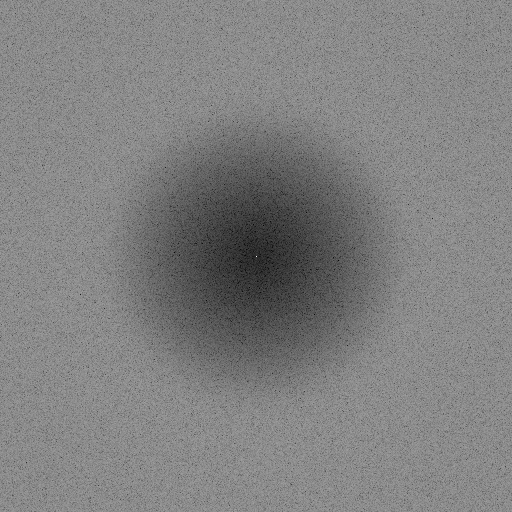
\includegraphics[width=\linewidth]{content/BlueNoise/Bilder/FFT_LDR_LLL1_0.png}
        \caption{Fourier Spektrum $512^{2}$ blue noise Textur}
    \end{minipage}
\end{figure}



\subsubsection{Isotropie}
Die Isotropie(altgr. \textit{isos}-gleich und \textit{tropos}-Richtung)
einer blue noise Textur wird ausgenutzt. Dabei haben wir in allen
Dimensionen (in dieser Arbeit werden Texturen mit zwei benutzt) 
die Unabhängigkeit einer Eigenschaft. 

\begin{figure}[H]\label{pic:bayerPatternFFT}
    \centering
    \begin{minipage}[t]{0.45\linewidth}
        \centering
        
\includegraphics[width=\linewidth]{content/BlueNoise/Bilder/BayerMatrix.png}
        \caption{$512^{2}$ bayer pattern Textur}
    \end{minipage}
    \hfill
    \begin{minipage}[t]{0.45\linewidth}
        \centering
        
\includegraphics[width=\linewidth]{content/BlueNoise/Bilder/FFT_BayerMatrix.png}
        \caption{Fourier Spektrum $512^{2}$ bayer pattern Textur}
    \end{minipage}
\end{figure}

\subsubsection{Kachelung}
Möglichkeit der Kachelung. 
Eine weitere nützliche Eigenschaft der blue noise Verteilung ist die 
\begin{figure}[H]\label{pic:tiledBlueNoiseFFT}
    \centering
    \begin{minipage}[t]{0.45\linewidth}
        \centering
        
\includegraphics[width=\linewidth]{content/BlueNoise/Bilder/BlueNoise64Tiled.png}
        \caption{$512^{2}$ bayer pattern Textur}
    \end{minipage}
    \hfill
    \begin{minipage}[t]{0.45\linewidth}
        \centering
        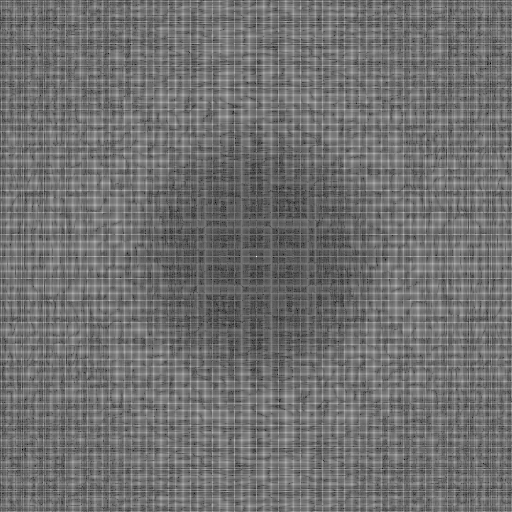
\includegraphics[width=\linewidth]{content/BlueNoise/Bilder/FFT_BlueNoise64Tiled.png}
        \caption{Fourier Spektrum $512^{2}$ bayer pattern Textur}
    \end{minipage}
\end{figure}